\documentclass[11pt]{article}
\usepackage[letterpaper,margin=0.5in,nohead,nofoot]{geometry}
\usepackage{color}
\usepackage{amsfonts}
\usepackage{amssymb}
\usepackage{amsmath}
\usepackage{setspace}
\usepackage{graphicx}


\everymath{\displaystyle}
\onehalfspacing

%\newcommand{\bra}[1]{\langle #1|}
%\newcommand{\ket}[1]{|#1\rangle}
\newcommand{\braket}[2]{\langle #1|#2\rangle}
\mathchardef\minus = "002D

\newcommand{\swY}[4][]{{}_{{}_{#2}}\!Y^{#1}_{#3}(#4)}
\newcommand{\swSH}[5][]{{}_{{}_{#2}}S^{#1}_{#3}(#4;#5)}
\newcommand{\swS}[5][]{{}_{{}_{#2}}S^{#1}_{#3}(#4;#5)}
\newcommand{\scA}[4][]{{}_{{}_{#2}}A^{#1}_{#3}(#4)}
\newcommand{\YSH}[3][]{\mathcal{A}^{#1}_{#2}(#3)}

\begin{document}
\noindent{\large\bf Quasi-normal Mode Decomposition for the ring-down} \\

\noindent
Teukolsky general field solution:
\begin{equation}
\psi(t,r,\theta,\phi) = \frac{1}{2\pi} \int {e^{-i\omega t} \sum_{\ell,m} \swSH{s}{\ell{m}}{\theta,\phi}{a\omega}R_{\ell{m}}(r) d\omega },
\end{equation}
where the summation over $\ell$ and $m$ is always confined to $|s|<
\ell < \infty$ and $|m| \leq \ell$. To represent outgoing
gravitational waves, we use $s=-2$ and $\psi = \rho^{-4}\Psi_4$, with
$\Psi_4$ being the Weyl scalar that behaves like an 
outgoing gravitational wave at large distances and $\rho\equiv-1/(r-ia\cos\theta)$.
Asymptotically, $R_{lm}(r)=r^3e^{i\omega r^*}$ ($r^*$ is the
''tortoise'' radial coordinate), $\rho=1/r$, and we find
\begin{equation}
\Psi_4 \sim \frac1{r}\frac{1}{2\pi} \int {e^{-i\omega (t-r^*)} \sum_{\ell,m} \swSH{\minus 2}{\ell{m}}{\theta,\phi}{a\omega} d\omega }.
\end{equation}
Making both sides dimensionless, we take as our general asymptotic expansion for outgoing gravitational waves:
\begin{equation}
rM\Psi_4 = \frac{M}{2\pi} \int {e^{-i\omega (t-r^*)} \sum_{\ell,m} \swSH{\minus 2}{\ell{m}}{\theta,\phi}{a\omega} d\omega }.
\end{equation}

To represent the ring-down of a Kerr black hole, we replace the
Fourier integral with a QNM expansion (a careful assumption, because
QNMs are not a complete set).  For each mode $(\ell,m)$, there are
two infinite sets of QNMs labeled by $n$: $\bar\omega_{\ell{m}n}$ and
$\bar\omega^\prime_{\ell{m}n}$.  The $n=0$ modes represent the
dominant QNM for each $(\ell,m)$, and the higher values of $n$
represent overtones.  When we replace the integral with a sum over all QNM, we must include both sets of modes:
\begin{equation}
rM\Psi_4 = \sum_{\ell{m}n}\left\{C_{\ell{m}n}e^{-i\bar\omega_{\ell{m}n} (t-r^*)}
           \swSH{\minus 2}{\ell{m}}{\theta,\phi}{a\bar\omega_{\ell{m}n}} 
           + C^\prime_{\ell{m}n}e^{-i\bar\omega^\prime_{\ell{m}n} (t-r^*)}
           \swSH{\minus 2}{\ell{m}}{\theta,\phi}{a\bar\omega^\prime_{\ell{m}n}}
           \right\}, 
\end{equation}
where $C_{\ell{m}n}$ and $C^\prime_{\ell{m}n}$ are the arbitrary
dimensionless complex coefficients of the QNM expansion.

The two sets of QNMs for Kerr are closely related to each other.  The $\bar\omega$ correspond to ``positive frequency'' modes and the $\bar\omega^\prime$ to ``negative frequency'' modes in the following sense.  Let us define:
\begin{align}
    \bar\omega_{\ell{m}n} &\equiv 
    \omega_{\ell{m}n} - \frac{i}{\tau_{\ell{m}n}}
      &;\quad a\bar\omega_{\ell{m}n}\equiv c_{\ell{m}n}
    &\quad:\quad\mbox{and}\quad \omega_{\ell{m}n} \ge 0, \\
    \bar\omega^\prime_{\ell{m}n} &\equiv 
    \omega^\prime_{\ell{m}n} - \frac{i}{\tau^\prime_{\ell{m}n}}
      &;\quad a\bar\omega^\prime_{\ell{m}n}\equiv c^\prime_{\ell{m}n}
    &\quad:\quad\mbox{and}\quad \omega^\prime_{\ell{m}n} \le 0.
\end{align}
They are further related by the fact that:
\begin{align}
\omega^\prime_{\ell{m}n} = -\omega_{\ell(-m)n} \\
\tau^\prime_{\ell{m}n} = \tau_{\ell(-m)n}.
\end{align} 
In terms of these definitions, and assuming we evaluate the expansion at fixed $r$ and $r^*$, we find:
\begin{equation}
rM\Psi_4 = \sum_{\ell{m}n} \left\{ C_{\ell{m}n} e^{-i\omega_{\ell{m}n}t}e^{-t/\tau_{\ell{m}n}} \swSH{\minus 2}{\ell{m}}{\theta,\phi}{c_{\ell{m}n}} + C^\prime_{\ell{m}n} e^{i\omega_{\ell(-m)n}}e^{-t/\tau_{\ell(-m)n}} \swSH{\minus 2}{\ell{m}}{\theta,\phi}{c^\prime_{\ell{m}n}} \right\},
\end{equation}
where we have absorbed constant factors involving $e^{r^*}$ into the
expansion coefficients.

Using the fact that the sum over $m$ extends from $-\ell\cdots\ell$, we can trivially rewrite the expansion as:
\begin{equation}
rM\Psi_4 = \sum_{\ell{m}n} \left\{ C_{\ell{m}n} e^{-i\omega_{\ell{m}n}t}e^{-t/\tau_{\ell{m}n}} \swSH{\minus 2}{\ell{m}}{\theta,\phi}{c_{\ell{m}n}} + C^\prime_{\ell(-m)n} e^{i\omega_{\ell{m}n}}e^{-t/\tau_{\ell{m}n}} \swSH{\minus 2}{\ell(-m)}{\theta,\phi}{c^\prime_{\ell(-m)n}} \right\}.
\end{equation}
Furthermore, because
\begin{equation}
c^\prime_{\ell(-m)n} = a\left(\omega^\prime_{\ell(-m)n} 
               - \frac{i}{\tau^\prime_{\ell(-m)n}}\right) =
               -a\left(\omega_{\ell{m}n} 
               - \frac{i}{\tau_{\ell{m}n}}\right)^* = -c^*_{\ell{m}n},
\end{equation}
and by the symmetries of the spin-weighted spheroidal harmonics given in Eqns~(\ref{eqn:swSHminuss}) and (\ref{eqn:swSHminusm}), we find
\begin{equation}
\swSH{\minus 2}{\ell(-m)}{\theta,\phi}{c^\prime_{\ell(-m)n}} = (-1)^l \swSH[*]{\minus 2}{\ell{m}}{\pi-\theta,\phi}{c_{\ell{m}n}},
\end{equation}

\noindent
Plugging those in, we get
\begin{equation}
\nonumber rM\Psi_4 = \sum_{\ell{m}n} \left\{C_{\ell{m}n} e^{-i\omega_{\ell{m}n}t}e^{-t/\tau_{\ell{m}n}} \swSH{\minus 2}{\ell{m}}{\theta,\phi}{c_{\ell{m}n}}
  + (-1)^\ell C^\prime_{\ell(-m)n} e^{i\omega_{\ell{m}n}t}e^{-t/\tau_{\ell{m}n}} \swSH[*]{\minus 2}{\ell{m}}{\pi-\theta,\phi}{c_{\ell{m}n}} \right\}.
\end{equation}
Finally, we can rewrite the two complex expansion coefficients as
\begin{align}
  C_{\ell{m}n} &\equiv A_{\ell{m}n}e^{i\phi_{\ell{m}n}}, \\
  C^\prime_{\ell(-m)n} &\equiv (-1)^\ell A^\prime_{\ell{m}n}e^{i\phi^\prime_{\ell{m}n}},
\end{align}
where $A_{\ell{m}n}$, $A^\prime_{\ell{m}n}$, $\phi_{\ell{m}n}$ and $\phi^\prime_{\ell{m}n}$ are real parameters.  The resulting equation is:
\begin{align} \label{eqn:Psi4SH:expan}
\nonumber rM\Psi_4 &= \sum_{\ell{m}n} \Bigl\{A_{\ell{m}n} e^{-i\omega_{\ell{m}n}t+i\phi_{\ell{m}n}}e^{-t/\tau_{\ell{m}n}} \swSH{\minus 2}{\ell{m}}{\theta,\phi}{c_{\ell{m}n}} \nonumber\\ & {} \hspace{0.5in}
  + A^\prime_{\ell{m}n} e^{i\omega_{\ell{m}n}t+i\phi^\prime_{\ell{m}n}}e^{-t/\tau_{\ell{m}n}} \swSH[*]{\minus 2}{\ell{m}}{\pi-\theta,\phi}{c_{\ell{m}n}} \Bigr\}.
\end{align}

\noindent\\
On the other hand, the Weyl scalar can also be decomposed using spin-weight $\minus 2$ spherical harmonics.  Again, assuming fixed $r$ and $r^*$:
\begin{equation}\label{eqn:Psi4Y:expan}
rM\Psi_4 = \sum_{\ell{m}} C_{\ell{m}}(t) \swY{\minus 2}{\ell{m}}{\theta,\phi},
\end{equation} 
The next step is to relate complex amplitudes $C_{\ell{m}}$ to the parameters of the ring-down signal (\ref{eqn:Psi4SH:expan}).  To accomplish this, we first expand the spheroidal harmonics in terms of spherical harmonics:
\begin{equation} \label{eqn:swSH:expan}
\swSH{\minus 2}{\ell{m}}{\theta,\phi}{c} = \sum_{\ell^\prime} \YSH{\ell^\prime\ell{m}}{c} \swY{\minus 2}{\ell^\prime{m}}{\theta,\phi}.
\end{equation}
Using Eqns~(\ref{eqn:swYminuss}), (\ref{eqn:swYminusm}), (\ref{eqn:swSHminuss}), and (\ref{eqn:swSHminusm}), we also have
\begin{equation} \label{eqn:swSconj:expan}
\swSH[*]{\minus 2}{\ell{m}}{\pi-\theta,\phi}{c} = \sum_{\ell^\prime} (-1)^{\ell^\prime}\YSH[*]{\ell^\prime\ell{m}}{c} \swY{\minus 2}{\ell^\prime(-m)}{\theta,\phi}.
\end{equation}
[Note: $\YSH[*]{\ell^\prime\ell{m}}{c} = (-1)^{\ell^\prime+\ell}\YSH{\ell^\prime\ell(-m)}{-c^*}$.]

So, equating Eqs.~(\ref{eqn:Psi4SH:expan}) and (\ref{eqn:Psi4Y:expan}), 
\begin{equation} \label{eqn:equate:expan}
\begin{aligned}
\sum_{\ell{m}} C_{\ell{m}}(t) \swY{\minus 2}{\ell{m}}{\theta,\phi} & = \sum_{\ell{m}n} \Big\{ A_{\ell{m}n} e^{-i\omega_{\ell{m}n}t+i\phi_{\ell{m}n}}e^{-t/\tau_{\ell{m}n}} \swSH{\minus 2}{\ell{m}}{\theta,\phi}{c_{\ell{m}n}}\\
& + A^\prime_{\ell{m}n} e^{i\omega_{\ell{m}n}t+i\phi^\prime_{\ell{m}n}}e^{-t/\tau_{\ell{m}n}} \swSH[*]{\minus 2}{\ell{m}}{\pi-\theta,\phi}{c_{\ell{m}n}} \Big\},
\end{aligned}
\end{equation}
and using the usual definition for the inner product $\braket{f(\theta, \phi)}{g(\theta, \phi)} \equiv \int{f^{*}(\theta, \phi) g(\theta, \phi) d\Omega}$ along with the orthonormality of the spin-weighted spherical harmonics, Eq,~(\ref{eqn:equate:expan}) becomes
\begin{equation} \label{clm:eq2}
\begin{aligned}
C_{\ell^\prime{m^\prime}}(t) &= \sum_{\ell{m}n} \Big\{ 
   A_{\ell{m}n} e^{-i\omega_{\ell{m}n}t+i\phi_{\ell{m}n}}e^{-t/\tau_{\ell{m}n}} 
   \braket{\swY{\minus 2}{\ell^\prime{m^\prime}}{\theta,\phi}}{\swSH{\minus 2}{\ell{m}}{\theta,\phi}{c_{\ell{m}n}}} \\
& {}\hspace{0.5in} 
  + A^\prime_{\ell{m}n} e^{i\omega_{\ell{m}n}t+i\phi^\prime_{\ell{m}n}}e^{-t/\tau_{\ell{m}n}} 
   \braket{\swY{\minus 2}{\ell^\prime{m^\prime}}{\theta,\phi}}{\swSH[*]{\minus 2}{\ell{m}}{\pi-\theta,\phi}{c_{\ell{m}n}}} \Big\}.
\end{aligned}
\end{equation}

\noindent
Finally, using the expansion in Eqs.~(\ref{eqn:swSH:expan}) and (\ref{eqn:swSconj:expan}), and
the orthonormality of the spin-weighted spherical harmonics we get
\begin{equation}
\begin{aligned} \label{clm:eq3}
C_{\ell^\prime{m}^\prime}(t) & = \sum_{\ell{m}n} \Big\{ 
   A_{\ell{m}n} e^{-i\omega_{\ell{m}n}t+i\phi_{\ell{m}n}}e^{-t/\tau_{\ell{m}n}}
    \sum_{\ell^{\prime\prime}} \YSH{\ell^{\prime\prime}\ell{m}}{c_{\ell{m}n}}
    \braket{\swY{\minus 2}{\ell^\prime{m}^\prime}{\theta,\phi}}{\swY{\minus 2}{\ell^{\prime\prime}m}{\theta,\phi}} \\
& {} \hspace{0.6in}
  + A^\prime_{\ell{m}n} e^{i\omega_{\ell{m}n}t+i\phi^\prime_{\ell{m}n}}e^{-t/\tau_{\ell{m}n}}
    \sum_{\ell^{\prime\prime}} (-1)^{\ell^{\prime\prime}} \YSH[*]{\ell^{\prime\prime}\ell{m}}{c_{\ell{m}n}}
    \braket{\swY{\minus 2}{\ell^\prime{m}^\prime}{\theta,\phi}}{\swY{\minus 2}{\ell^{\prime\prime}(-m)}{\theta,\phi}} \Big\} \\ 
 & = \sum_{\ell{n}} \Big\{ 
   A_{\ell{m^\prime}n} e^{-i\omega_{\ell{m^\prime}n}t+i\phi_{\ell{m^\prime}n}}e^{-t/\tau_{\ell{m^\prime}n}}
    \YSH{\ell^\prime\ell{m^\prime}}{c_{\ell{m^\prime}n}} \\
& {} \hspace{0.6in}
  + (-1)^{\ell^\prime}A^\prime_{\ell(-m^\prime)n} e^{i\omega_{\ell(-m^\prime)n}t+i\phi^\prime_{\ell(-m^\prime)n}}e^{-t/\tau_{\ell(-m^\prime)n}}
    \YSH[*]{\ell^\prime\ell(-m^\prime)}{c_{\ell(-m^\prime)n}} \Big\}.
\end{aligned}
\end{equation}
After relabeling indices we have
\begin{equation}\label{eq:SphericalKerrModes}
\begin{aligned}
 C_{\ell{m}}(t) & = \sum_{\ell^\prime{n}} \Big\{ 
   A_{\ell^\prime{m}n}\YSH{\ell\ell^\prime{m}}{c_{\ell^\prime{m}n}}
    e^{-i\omega_{\ell^\prime{m}n}t+i\phi_{\ell^\prime{m}n}}e^{-t/\tau_{\ell^\prime{m}n}} \\
& {} \hspace{0.6in}
  + (-1)^\ell A^\prime_{\ell^\prime(-m)n}
    \YSH[*]{\ell\ell^\prime(-m)}{c_{\ell^\prime(-m)n}}
    e^{i\omega_{\ell^\prime(-m)n}t+i\phi^\prime_{\ell^\prime(-m)n}}e^{-t/\tau_{\ell^\prime(-m)n}} \Big\}.
\end{aligned}
\end{equation}
Finally, let us define two new functions:
\begin{align}
  \mathcal{R}_{\ell\ell^\prime{m}n}(t,\phi) &\equiv 
    \YSH{\ell\ell^\prime{m}}{c_{\ell^\prime{m}n}}
    e^{-i\omega_{\ell^\prime{m}n}t+i\phi_{\ell^\prime{m}n}}e^{-t/\tau_{\ell^\prime{m}n}}, \\
  \mathcal{R}^\prime_{\ell\ell^\prime{m}n}(t,\phi) &\equiv  
    (-1)^\ell\YSH[*]{\ell\ell^\prime{m}}{c_{\ell^\prime{m}n}}
    e^{i\omega_{\ell^\prime{m}n}t+i\phi{\ell^\prime{m}n}}e^{-t/\tau_{\ell^\prime{m}n}}.
\end{align}
So,
\begin{equation}
 C_{\ell{m}}(t) = \sum_{\ell^\prime{n}} \left\{ 
   A_{\ell^\prime{m}n}\mathcal{R}_{\ell\ell^\prime{m}n}(t,\phi_{\ell^\prime{m}n})
  + A^\prime_{\ell^\prime(-m)n}
     \mathcal{R}^\prime_{\ell\ell^\prime(-m)n}(t,\phi^\prime_{\ell^\prime(-m)n})
     \right\}.
\end{equation}
Thus, for each $\ell$ and $m$ we have four numbers $A_{\ell^\prime{m}n}$, $A^\prime_{\ell^\prime(-m)n}$, $\phi_{\ell^\prime{m}n}$, and $\phi^\prime_{\ell^\prime(-m)n}$ describing the wave, which later will be exploited as fit parameters.

\newpage
\noindent{\large\bf Appendix: Spin-Weighted Spheroidal Harmonics}
\vspace{0.25in}

The spin-weighted spheroidal harmonics,
$\swSH{s}{\ell{m}}{\theta,\phi}{c}$, are generalizations of the
spin-weighted spherical harmonics,
$\swY{s}{\ell{m}}{\theta,\phi}=\swSH{s}{\ell{m}}{\theta,\phi}{0}$,
where $s$ is the spin weight of the harmonic, and $c$ is the
oblateness parameter.  The angular dependence separates as
\begin{equation}
  \swSH{s}{\ell{m}}{\theta,\phi}{c} \equiv 
  \frac1{2\pi}\,\swS{s}{\ell{m}}{\cos\theta}{c}e^{im\phi}.
\end{equation}
With $x\equiv\cos\theta$, the spin-weighted spheroidal {\em function},
$\swS{s}{\ell{m}}{x}{c}$, satisfies
\begin{equation}\label{eqn:swSF_DiffEqn}
\partial_x \Big[ (1-x^2)\partial_x [\swS{s}{\ell{m}}{x}{c}]\Big] 
    + \bigg[(cx)^2 - 2 csx + s + \scA{s}{\ell m}{c} 
      - \frac{(m+sx)^2}{1-x^2}\bigg]\swS{s}{\ell{m}}{x}{c} = 0,
\end{equation}
where $\scA{s}{\ell m}{c}$ is the separation constant.

The basic symmetries inherent in the spin-weighted spheroidal functions
follow from~(\ref{eqn:swSF_DiffEqn}):
\begin{eqnarray}
s\rightarrow-s;\ x\rightarrow-x &\Rightarrow&
    \left\{\begin{array}{c}\swS{-s}{\ell{m}}{x}{c}\propto\swS{s}{\ell{m}}{-x}{c} \\
        \scA{-s}{\ell{m}}{c} = \scA{s}{\ell{m}}{c} + 2s \end{array}\right. \\
m\rightarrow-m;\ x\rightarrow-x;\ c\rightarrow-c &\Rightarrow&
    \left\{\begin{array}{c}\swS{s}{\ell(-m)}{x}{c}\propto\swS{s}{\ell{m}}{-x}{-c}\\
        \scA{s}{\ell(-m)}{c} = \scA{s}{\ell{m}}{-c} \end{array}\right. \\
\mbox{complex conjugation} &\Rightarrow&
    \left\{\begin{array}{c} \swS[*]{s}{\ell{m}}{x}{c}\propto\swS{s}{\ell{m}}{x}{c^*} \\
        \scA[*]{s}{\ell{m}}{c} = \scA{s}{\ell{m}}{c^*} \end{array}\right.
\end{eqnarray}

Additional sign and normalization conventions are chosen for
consistency with common sign conventions for the angular-spheroidal
functions, $\swS{}{\ell{m}}{x}{c} = \swS{0}{\ell{m}}{x}{c}$, and the
spin-weighted spheroidal harmonics, $\swY{s}{\ell{m}}{\theta,\phi}$.

\vspace{0.25in}
\noindent
{\it Angular spheroidal functions}
\begin{equation}
\partial_x \Big[ (1-x^2)\partial_x \swS{}{\ell{m}}{x}{c}\Big] + \bigg[(cx)^2 + \scA{}{\ell{m}}{c} - \frac{m^2}{1-x^2}\bigg]\swS{}{\ell{m}}{x}{c} = 0
\end{equation}
\begin{align}
\swS{}{\ell{m}}{-x}{c} &= (-1)^{\ell+m}\swS{}{\ell{m}}{x}{c}& \\
\swS{}{\ell{m}}{x}{-c} &= \swS{}{\ell{m}}{x}{c} 
           &:\ \scA{}{\ell{m}}{-c} = \scA{}{\ell{m}}{c} \\
\swS{}{\ell(-m)}{x}{c} &= (-1)^m\swS{}{\ell{m}}{x}{c} 
           &:\ \scA{}{\ell(-m)}{c} = \scA{}{\ell{m}}{c} \\
\swS[*]{}{\ell{m}}{x}{c} &= \swS{}{\ell{m}}{x}{c^*} 
           &:\ \scA[*]{}{\ell{m}}{c} = \scA{}{\ell{m}}{c^*}
\end{align}

\noindent
{\it Spin-weighted spherical functions}
\begin{equation}\label{Eqn:swSF:Diff_eqn0}
\partial_x \Big[ (1-x^2)\partial_x [\swS{s}{\ell{m}}{x}{0}]\Big] + \bigg[s + \scA{s}{\ell{m}}{0} - \frac{(m+sx)^2}{1-x^2}\bigg]\swS{s}{\ell{m}}{x}{0} = 0
\end{equation}
\begin{equation}\label{eqn:scA_spherical}
\scA{s}{\ell{m}}{0} = l(l+1) - s(s+1)\\
\end{equation}
\begin{align}
\swS{-s}{\ell{m}}{x}{0} &= (-1)^{\ell+m}\swS{s}{\ell{m}}{-x}{0} 
           &:\ \scA{-s}{\ell{m}}{0} = \scA{s}{\ell{m}}{0} + 2s \\
\swS{s}{\ell(-m)}{x}{0} &= (-1)^{\ell+s}\swS{s}{\ell{m}}{-x}{0} 
           &:\ \scA{s}{\ell(-m)}{0} = \scA{s}{\ell{m}}{0} \\
\swS[*]{s}{\ell{m}}{x}{0} &= \swS{s}{\ell{m}}{x}{0} 
           &:\ \scA[*]{s}{\ell{m}}{0} = \scA{s}{\ell{m}}{0}
\end{align}

\noindent
{\it Spin-weighted spherical harmonics}
\begin{align}\label{eqn:swYminuss}
\swY{-s}{\ell{m}}{\theta,\phi}=(-1)^{\ell+m}\swY{s}{\ell{m}}{\pi-\theta,\phi} \\ \label{eqn:swYminusm}
\swY{s}{\ell(-m)}{\theta,\phi}=(-1)^{s+m}\swY[*]{-s}{\ell{m}}{\theta,\phi}
\end{align}

\noindent
These leave us with the following conventions for the spin-weighted spherical harmonics and spheroidal functions:
\begin{align}
\swS{-s}{\ell{m}}{x}{c} &= (-1)^{\ell+m}\swS{s}{\ell{m}}{-x}{c} 
           &:\ \scA{-s}{\ell{m}}{c} = \scA{s}{\ell{m}}{c} + 2s \\
\swS{s}{\ell(-m)}{x}{c} &= (-1)^{\ell+s}\swS{s}{\ell{m}}{-x}{-c} 
           &:\ \scA{s}{\ell(-m)}{c} = \scA{s}{\ell{m}}{-c} \\
\swS[*]{s}{\ell{m}}{x}{c} &= \swS{s}{\ell{m}}{x}{c^*} 
           &:\ \scA[*]{s}{\ell{m}}{c} = \scA{s}{\ell{m}}{c^*}
\end{align}
\begin{align}\label{eqn:swSHminuss}
\swSH{-s}{\ell{m}}{\theta,\phi}{c} &= (-1)^{\ell+m}\swSH{s}{\ell{m}}{\pi-\theta,\phi}{c} \\ \label{eqn:swSHminusm}
\swSH{s}{\ell(-m)}{\theta,\phi}{c} &= (-1)^{s+m}\swSH[*]{-s}{\ell{m}}{\theta,\phi}{-c^*}
\end{align}

\newpage
\noindent{\large\bf Appendix: Spin-Weighted Spherical Harmonics}
\vspace{0.25in}

\begin{equation}
  \swY{s}{\ell{m}}{\theta,\phi} \equiv 
  \frac1{2\pi}\,\swS{s}{\ell{m}}{\cos\theta}{0}e^{im\phi}
  = (-1)^s\sqrt{\frac{2\ell+1}{4\pi}}d^\ell_{m(-s)}(\theta)e^{im\phi},
\end{equation}
where $d^\ell_{mn}(\theta)$ is the Wigner d-function defined by
\begin{equation}
  d^\ell_{mn}(\theta) \equiv (-1)^\lambda
       \left(\begin{array}{c}2\ell-k \\ k+a \end{array}\right)^{\frac12}
       \left(\begin{array}{c}k+b \\ b \end{array}\right)^{-\frac12}
       \left(\sin\frac\theta2\right)^a
       \left(\cos\frac\theta2\right)^b
       P^{(a,b)}_k(\cos\theta),
\end{equation}
where $k\equiv \min(\ell+n,\ell-n,\ell+m,\ell-m)$ and
\begin{align}
  \mbox{if\ }k &= \left\{\begin{array}{ccll}
           \ell+n &:& a=m-n, & \lambda = m-n \\
           \ell-n &:& a=n-m, & \lambda = 0 \\
           \ell+m &:& a=n-m, & \lambda = 0 \\
           \ell-m &:& a=m-n, & \lambda = m-n \end{array}\right. \\
     b &= 2\ell-2k-a.
\end{align}
\begin{center}
\fbox{\parbox{6in}{
More generally, when a non-vanishing spin-gauge $\gamma$ is allowed,
\[
  \swY[\gamma]{s}{\ell{m}}{\theta,\phi}
  = (-1)^s\sqrt{\frac{2\ell+1}{4\pi}}
           \left(D^\ell_{m(-s)}(\phi,\theta,-\gamma)\right)^*,
\]
where the Wigner rotation matrices $D^\ell_{mn}(\phi,\theta,\gamma)$
is defined by
\[
  D^\ell_{mn}(\phi,\theta,\gamma) \equiv 
       e^{-im\phi} d^\ell_{mn}(\theta) e^{-in\gamma}.
\]
}}
\end{center}

The spin-weighted spherical functions, $\swS{s}{\ell{m}}{x}{0}$, 
satisfy the recurrence relations
\begin{equation}\label{eqn:swS:xrecur}
  x \swS{s}{\ell{m}}{x}{0} = 
       \mathcal{F}_{s\ell{m}} \swS{s}{(\ell+1){m}}{x}{0}
       + \mathcal{G}_{s\ell{m}} \swS{s}{(\ell-1){m}}{x}{0}
       + \mathcal{H}_{s\ell{m}} \swS{s}{\ell{m}}{x}{0},
\end{equation}
where
\begin{align}
  \label{eqn:x1coefF}
  \mathcal{F}_{s\ell{m}} &= \left\{\begin{array}{rcl}
       \mbox{if\ }s\ne0 &:& 
       \sqrt{\frac{(\ell+1)^2-m^2}{(2\ell+3)(2\ell+1)}}
       \sqrt{\frac{(\ell+1)^2-s^2}{(\ell+1)^2}}, \\
       \mbox{if\ }s=0 &:& 
       \sqrt{\frac{(\ell+1)^2-m^2}{(2\ell+3)(2\ell+1)}},
       \end{array}\right. \\
  \label{eqn:x1coefG}
  \mathcal{G}_{s\ell{m}} &= \left\{\begin{array}{rcl}
       \mbox{if\ }\ell\ne0 &:& 
       \sqrt{\frac{\ell^2-m^2}{4\ell^2-1}}
       \sqrt{\frac{\ell^2-s^2}{\ell^2}}, \\
       \mbox{if\ }\ell=0 &:& 0, 
       \end{array}\right. \\
  \label{eqn:x1coefH}
  \mathcal{H}_{s\ell{m}} &= \left\{\begin{array}{rcl}
       \mbox{if\ }\ell\ne0 \mbox{\ and\ } s\ne0 &:& 
       -\frac{ms}{\ell(\ell+1)}, \\
       \mbox{if\ }\ell=0 \mbox{\ or\ } s=0 &:& 0.
       \end{array}\right.
\end{align}
\begin{align}\label{eqn:swS:x2recur}
  x^2 \swS{s}{\ell{m}}{x}{0} &= 
       \mathcal{A}_{s\ell{m}} \swS{s}{(\ell+2){m}}{x}{0}
       + \mathcal{B}_{s\ell{m}} \swS{s}{\ell{m}}{x}{0}
       + \mathcal{C}_{s\ell{m}} \swS{s}{(\ell-2){m}}{x}{0} \nonumber \\
       &{}\hspace{0.5in}
       + \mathcal{D}_{s\ell{m}} \swS{s}{(\ell+1){m}}{x}{0}
       + \mathcal{E}_{s\ell{m}} \swS{s}{(\ell-1){m}}{x}{0},
\end{align}
where
\begin{align}\label{eqn:x2coefA}
  \mathcal{A}_{s\ell{m}} &= \mathcal{F}_{s\ell{m}}\mathcal{F}_{s(\ell+1)m}, \\
  \label{eqn:x2coefD}
  \mathcal{D}_{s\ell{m}} &= \mathcal{F}_{s\ell{m}}
         (\mathcal{H}_{s(\ell+1)m} + \mathcal{H}_{s\ell{m}}) , \\
  \label{eqn:x2coefB}
  \mathcal{B}_{s\ell{m}} &= \mathcal{F}_{s\ell{m}}\mathcal{G}_{s(\ell+1)m}
     + \mathcal{G}_{s\ell{m}}\mathcal{F}_{s(\ell-1)m} 
     + \mathcal{H}^2_{s\ell{m}}, \\
  \label{eqn:x2coefE}
  \mathcal{E}_{s\ell{m}} &= \mathcal{G}_{s\ell{m}}
         (\mathcal{H}_{s(\ell-1)m} + \mathcal{H}_{s\ell{m}}) , \\
  \label{eqn:x2coefC}
  \mathcal{C}_{s\ell{m}} &= \mathcal{G}_{s\ell{m}}\mathcal{G}_{s(\ell-1)m}.
\end{align}

\newpage
\noindent{\large\bf Appendix: Lorentz Transformations with
  Spin-Weighted Spherical Harmonics}\\ {\em See Goldberg et.\ a,l
  ``Spin-s Spherical Harmonics and $\eth$'', J.\ Math.\ Phys., 1967,
  {\bf 8}, 2155;\\ Newman \& Penrose, ``Note on the
  Bondi-Metzner-Sachs Group'', J.\ Math.\ Phys., 1966, {\bf 7}, 863;\\
  Morrison \& Parker, ``A Guide to Rotations in Quantum Mechanics'',
  Aust.\ J.\ PHys., 1987, {\bf 40}, 465.}
\vspace{0.25in}

Care must be taken when considering coordinate transformations when
spin-wighted tensors are used.  Start with a standard spherical
coordinate system $(\theta,\phi)$ with metric ${\rm d}s^2={\rm
  d}\theta^2+\sin^2\theta{\rm d}\phi^2$.  To consider spin-weighted
functions, we need to define a complex vector $\vec{m}$, so that
$\vec{m}$ and its conjugate $\vec{m}^*$ form a null basis dyad for
vectors satisfying $\vec{m}\cdot\vec{m}=0$ and
$\vec{m}\cdot\vec{m}^*=1$.  $\vec{m}$ is thus defined only up to a
phase factor, so $\vec{m}^\prime=e^{i\psi}\vec{m}$.  A quantity is
said to tranform with spin-weight $s$ if it tranforms as
$\eta^\prime=e^{is\psi}\eta$.

In spherical coordinates, a standard definition is to take
\begin{equation}
  \vec{m} = \frac1{\sqrt2}(\partial_\theta + \frac{i}{\sqrt\theta}\partial_\phi)
\quad\mbox{and}\quad
  \tilde{m} = \frac1{\sqrt2}({\rm d}\theta + i\sqrt\theta{\rm d}\phi),
\end{equation}
where $\tilde{m}$ is the basis form dual to $\vec{m}$.  With this
definition, the ${\rm Re}{\vec{m}}$ is tangent to curves of constant
$\phi$, and the ${\rm Im}{\vec{m}}$ is tangent to curves of constant
$\theta$.  To consider Lorentz transformations, it is convenient to
consider the complex coordinate transformation defined by
\begin{equation}
  \zeta\equiv e^{i\phi}\cot(\theta/2).
\end{equation}
We can then consider the complex pair $(\zeta,\zeta^2)$ as coordiantes
on the sphere and find the metric is given by
\begin{equation}
{\rm d}s^2 = \frac4{(1+\zeta\zeta^*)^2}{\rm d}\zeta{\rm d}\zeta^*.
\end{equation}
For clarity later on, we will let $\vec\mu$ denote the complex null
vector in this coordinate system.  It is natural to choose the ${\rm
  Re}{\vec\mu}$ to be tangent to curves of constant ${\rm Im}\zeta$
and the ${\rm Im}{\vec\mu}$ to be tangent to curves of constant ${\rm
  Re}\zeta$.  We can then write the $\tilde\mu$ as
\begin{equation}
  \tilde\mu = \frac1{\sqrt2}\frac2{1+\zeta\zeta^*}{\rm d}\zeta^*,
\end{equation}
and we find that
\begin{equation}
  \tilde{m} = e^{i(\phi+\pi)}\tilde\mu
\quad\mbox{and}\quad \vec{m} = e^{i(\phi+\pi)}\vec\mu.
\end{equation}
So, the two basis sets are related by a spin-rotation angle of $\phi+\pi$.

The effect of a proper, homogeneous Lorentz transformation can be
represented by the M\"{o}bius transformation
\begin{equation}\label{eq:Mobius-def}
  \acute\zeta = \frac{\alpha\zeta+\beta}{\gamma\zeta+\delta}
\quad\mbox{or}\quad
  \zeta = -\frac{\delta\acute\zeta-\beta}{\gamma\acute\zeta-\alpha}
\qquad\mbox{with}\qquad
\alpha\delta-\beta\gamma=1.
\end{equation}
Under this coordiate transformation, the metric becomes
\begin{equation}
  {\rm d}s^2 = K^2\frac4{(1+\acute\zeta\acute\zeta^*)^2}
              {\rm d}\acute\zeta{\rm d}\acute\zeta^*,
\end{equation}
where the conformal factor $K$ is defined by
\begin{equation}
  K\equiv \frac{|\alpha\zeta+\beta|^2+|\gamma\zeta+\delta|^2}{1+\zeta\zeta^*}.
\end{equation}
The complex null form in the $(\zeta^\prime,\zeta^{\prime*})$ coordinates,
$\tilde\mu^\prime$, is given by
\begin{equation}
  \tilde\mu^\prime = \frac1{\sqrt2}\frac{2K}{1+\acute\zeta\acute\zeta^*}
           {\rm d}\acute\zeta^*,
\end{equation}
and we find that
\begin{equation}
  \tilde\mu = e^{-i\Lambda}\tilde\mu^\prime
\quad\mbox{with}\quad e^{-i\Lambda}\equiv 
   \frac{\gamma\zeta+\delta}{\gamma^*\zeta^*+\delta^*} =
   \frac{\gamma^*\acute\zeta^*-\alpha^*}{\gamma\acute\zeta-\alpha}.
\end{equation}
So, the two basis sets are related by a spin-rotation angle of $-\Lambda$.

Finally, we can obtain the transformed $(\acute\theta,\acute\phi)$
coordinates from
\begin{equation}
  \acute\zeta\equiv e^{i\acute\phi}\cot(\acute\theta/2).
\end{equation}
The transformed metric is given by
\begin{equation}
{\rm d}s^2 = K^2({\rm d}\acute\theta^2+\sin^2\acute\theta{\rm d}\acute\phi^2).
\end{equation}
The complex null form in the $(\acute\theta,\acute\phi)$ coordinates,
$\tilde{m}^\prime$, is given by
\begin{equation}
\tilde{m}^\prime = \frac{K}{\sqrt2}
      ({\rm d}\acute\theta^2+\sin^2\acute\theta{\rm d}\acute\phi^2),
\end{equation}
and we find that
\begin{equation}
\tilde\mu^\prime = e^{-i(\acute\phi+\pi)}\tilde{m}^\prime.
\end{equation}
So, these two basis sets are related by a spin-rotation angle of
$-(\acute\phi+\pi)$.

To summarize:
\begin{equation}\label{eq:LorentzMetricTrans}
{\rm d}s^2 = {\rm d}\theta^2+\sin^2\theta{\rm d}\phi^2
     = \frac4{(1+\zeta\zeta^*)^2}{\rm d}\zeta{\rm d}\zeta^*
     =  K^2\frac4{(1+\acute\zeta\acute\zeta^*)^2}
              {\rm d}\acute\zeta{\rm d}\acute\zeta^*
     = K^2({\rm d}\acute\theta^2+\sin^2\acute\theta{\rm d}\acute\phi^2),
\end{equation}
and
\begin{equation}
\tilde{m} = e^{i(\phi+\pi)}\tilde\mu
     = e^{i(\phi-\Lambda+\pi)}\tilde\mu^\prime
     = e^{i(\phi-\acute\phi-\Lambda)}\tilde{m}^\prime.
\end{equation}
So, given a proper, homogeneous Lorentze transformation defined by the
M\"{o}bius transformation of Eq.~(\ref{eq:Mobius-def}), the metric
transforms by a conformal factor of $K^2$, and the complex null basis
includes a spin-rotation angle of $\phi-\acute\phi-\Lambda$.

To understand how spin-weighted spherical harmonics transform under 
Lorentz transformations, we note that (in terms of the $(\zeta,\zeta^*)$
coordinates) we can write these functions as
\begin{equation}
  \swY{s}{\ell m}{\zeta} = \sum_{m_1=0}^{L-s}{\sum_{m_2=0}^{L+s}{
      {}_sB^L_{\ell m}{}^{m_1m_2}{}_sZ^L_{m_1m_2}}}
\quad\mbox{where}\quad |s|\le\ell\le L,\quad |m|\le\ell,
\end{equation}
with
\begin{eqnarray}
 {}_sZ^L_{m_1m_2}&\equiv&(1+\zeta\zeta^*)^{-L}\zeta^{L-s-m_1}\zeta^{*L+s-m_2}, \\
{}_sB^L_{\ell m}{}^{m_1m_2} &\equiv&
    (-1)^{\ell+m}\sqrt{\frac{(\ell+m)!(\ell-m)!}{(\ell-s)!(\ell+s)!}
  \frac{(2\ell+1)}{4\pi}} \nonumber \\ &&\mbox{\hspace{0.25in}}
    \times\sum_{p=0}^{p_m}{(-1)^p
      \left(\begin{array}{c}\ell-s \\ p\end{array}\right)
        \left(\begin{array}{c}\ell+s \\ p+s-m\end{array}\right)
        \left(\begin{array}{c}L-\ell \\ L-s-m_1-p\end{array}\right)
          \delta_{m_2,m_1+s+m}}. \\ && \nonumber\\
    && p_m=\min(L-s-m_1,\ell-s,\ell+m),\quad
       0\le m_1\le L-s,\quad
       0\le m_2\le L+s\nonumber
\end{eqnarray}

The reason for this complicated representation of the ${}_sY_{\ell m}$
is that it is straightforward to show how the ${}_sZ^L_{m_1m_2}$
transform under the Lorentz transformation of Eq.~(\ref{eq:Mobius-def}),
\begin{equation}
{}_s\acute{Z}^L_{m_1m_2} = K^{-L}e^{is\Lambda}
    \sum_{n_1=0}^{L-s}{\sum_{n_2=0}^{L-s}{
        A^{[\frac12(L-s)][\frac12(L+s)]}_{m_1m_2;n_1n_2}{}_sZ^L_{n_1n_2}}}.
\end{equation}
So, up to a conformal factor $K^{-L}e^{is\Lambda}$, the functions
${}_sZ^L_{m_1m_2}$ transform under the
$\mathcal{D}^{[\frac12(L-s)][\frac12(L+s)]}$ irreducible
representation of the Lorentz group, and matrix elements of the
explicit representation are given by
$A^{(j_1)(j_2)}_{m_1m_2;n_1n_2}=A^{(j_1)}_{m_1n_1}A^{*(j_2)}_{m_2n_2}$
and
\begin{equation}
  A^{(j)}_{mn}=\sum_{p=0}^{\min(m,n)}{
    \alpha^{2j+p-m-n}\beta^{n-p}\gamma^{m-p}\delta^p
      \left(\begin{array}{c}2j-m \\ m-p\end{array}\right)
      \left(\begin{array}{c}m \\ p\end{array}\right)}.
\end{equation}

Because the ${}_sB^L_{\ell m}{}^{m_1m_2}$ form a square,
$(L-s+1)(L+s+1)$-dimensional, non-singular matrix, we find that
\begin{equation}
\swY{s}{\ell m}{\acute\zeta}=K^{-L}e^{is\Lambda}\sum_{\acute\ell\acute{m}}
         \mathcal{R}^{(s,L)}_{\ell m\acute\ell\acute{m}}
         \swY{s}{\acute\ell\acute{m}}{\zeta},
\end{equation}
where
\begin{equation}
  \mathcal{R}^{(s,L)}_{\ell m\acute\ell\acute{m}}\equiv
    \sum_{m_1,n_1=0}^{L-s} \sum_{m_2,n_2=0}^{L+s}
         {}_sB^L_{\ell m}{}^{m_1m_2}
         A^{[\frac12(L-s)][\frac12(L+s)]}_{m_1m_2;n_1n_2}
         \left( {}_sB^L_{\acute\ell\acute{m}}{}^{n_1n_2}\right)^{-1}.
\end{equation}
Transforming to the usual spherical coordiantes, we must remember to also
include the spin-rotation angles.  The result is
\begin{equation}\label{eq:LorentzYTrans}
\swY{s}{\ell m}{\acute\theta,\acute\phi}=
     K^{-L}e^{is(\Lambda-\phi+\acute\phi)}\sum_{\acute\ell\acute{m}}
         \mathcal{R}^{(s,L)}_{\ell m\acute\ell\acute{m}}
                 \swY{s}{\acute\ell\acute{m}}{\theta,\phi}.
\end{equation}
For general Lorentz transformations, the matrix
$\mathcal{R}^{(s,L)}_{\ell m\acute\ell\acute{m}}$ is dense.  However,
if we restrict outselves to rotations, then we find that the matrix is
block-diagonal and can be written as
\begin{equation}
  \mathcal{R}^{(s,L)}_{\ell m\acute\ell\acute{m}} = 
  D^\ell_{\acute{m}m}(\bar\alpha,\bar\beta,\bar\gamma)\delta_{\ell,\acute\ell}.
\end{equation}
Here, $\bar\alpha$, $\bar\beta$, and $\bar\gamma$ are the (real) Euler
angles defining the rotation (not to be confused with the (complex)
coefficients of the M\"{o}bius transformation).  These Euler angles
denote the angles in an active rotation taking the Cartesian basis
vectors of the un-primed coordinate system into the Cartesian basis
vectos of the primed coordiante system.  In other words, the
$\acute{z}$-axis will point in the $(\theta=\beta,\phi=\alpha)$
direction in the un-primed system.  The corresponding coefficients for
the M\"{o}bius transformation are
\begin{equation}
  \alpha = e^{-\frac{i}2(\bar\alpha+\bar\gamma)}\cos\tfrac{\bar\beta}2,
\quad
  \beta = e^{\frac{i}2(\bar\alpha-\bar\gamma)}\sin\tfrac{\bar\beta}2,
\quad
  \gamma = -\beta^*,
\quad
  \delta = \alpha^*. 
\end{equation}
Since $K=1$ for
rotations, this gives
\begin{equation}
\swY{s}{\ell m}{\acute\theta,\acute\phi}=
     e^{is(\Lambda-\phi+\acute\phi)}\sum_{\acute{m}}
         \swY{s}{\ell\acute{m}}{\theta,\phi}
         D^\ell_{\acute{m}m}(\bar\alpha,\bar\beta,\bar\gamma),
\end{equation}
which reduces to the usual transformation rule for spherical harmonics
when $s=0$.

We must consider two separate coordinate systems because the
spin-weighted spheroidal harmonics needed to describe the ring-down of
a Kerr Black hole are defined with respect to the direction of the
angular momentum of the black hole which may not align with the
$z$-axis of the ``code'' coordinates.

\noindent
\parbox[t]{3.5in}{\hrule height 0pt width 0pt
\setlength{\parindent}{0.25in}
Now, let the un-primed coordinate system $\{x,y,z\}$ be the ``code''
coordiante system, and let $(\theta,\phi)$ be the associated
coordinates on a 2-sphere of constant radius defined by the usual
transformation between Cartesian and spherical coordinates.  And, let
the primed coordinate system $\{\acute{x},\acute{y},\acute{z}\}$ be
the ``Kerr'' coordinate system with the $\acute{z}$-axis aligned with
the direction of the angular momentum of the Kerr black hole.

Let $\Psi_4(\theta,\phi)$ be the spin weight $s=-2$ Weyl scalar
containing the gravitational wave signal in the ``code'' frame.  In
the ``Kerr'' frame, it is given by
\begin{equation}
\Psi_4(\acute\theta,\acute\phi)=e^{i(-2)(\Lambda-\phi+\acute\phi)}\Psi_4(\theta,\phi)
\end{equation}
}
\parbox[t]{4in}{\hrule height 0pt width 0pt
\hspace{0.5in}
\begin{picture}(180,220)(0,0)
\put(0,0){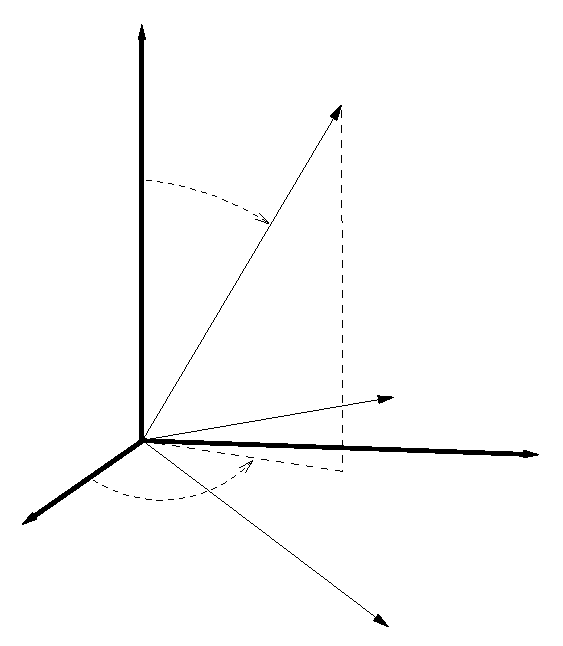
\includegraphics[width=2.5in,clip]{CoordRot}}
\put(0,27){$x$}
\put(175,51){$y$}
\put(37,209){$z$}
\put(128,3){$\acute{x}$}
\put(129,82){$\acute{y}$}
\put(103,181){$\acute{z}$}
\put(40,36){$\bar\alpha$}
\put(63,153){$\bar\beta$}
\end{picture}} 
Each scalar can be expanded in terms of its own set of spin-weighted
spherical harmonics:
\begin{equation}
\Psi_4(\theta,\phi)=\sum_{\ell m}C_{\ell m}\swY{-2}{\ell m}{\theta,\phi}
\qquad\mbox{and}\qquad
\Psi_4(\acute\theta,\acute\phi)=
\sum_{\ell m}\acute{C}_{\ell m}\swY{-2}{\ell m}{\acute\theta,\acute\phi}.
\end{equation}
This gives us
\begin{equation}
\Psi_4(\theta,\phi)=\sum_{\ell m}C_{\ell m}\swY{-2}{\ell m}{\theta,\phi}
=e^{-i(-2)(\Lambda-\phi+\acute\phi)}
\sum_{\ell m}\acute{C}_{\ell m}\swY{-2}{\ell m}{\acute\theta,\acute\phi}.
\end{equation}
Using the orthonormality of the spin-weighted spherical harmonics,
we find
\begin{equation}
C_{\acute\ell\acute{m}}=\oint{\swY[*]{-2}{\acute\ell\acute{m}}{\theta,\phi}
  \left(e^{-i(-2)(\Lambda-\phi+\acute\phi)}
  \sum_{\ell m}\acute{C}_{\ell m}\swY{-2}{\ell m}{\acute\theta,\acute\phi}\right)
  {\rm d}\Omega}
\end{equation}
Allowing for the moment that our coordinates are related by a proper,
homogeneous Lorentz transformation, we can use the inverse of
Eq.~(\ref{eq:LorentzYTrans})
\begin{equation}
\swY{s}{\ell m}{\theta,\phi}=
     K^Le^{-is(\Lambda-\phi+\acute\phi)}\sum_{\acute\ell\acute{m}}
         \mathcal{R}^{-1(s,L)}_{\ell m\acute\ell\acute{m}}
                 \swY{s}{\acute\ell\acute{m}}{\acute\theta,\acute\phi} 
\end{equation}
and transform the area element using Eq.~(\ref{eq:LorentzMetricTrans}) to
get
\begin{eqnarray}
C_{\acute\ell\acute{m}}&=&\oint{
  \left(K^Le^{-i(-2)(\Lambda-\phi+\acute\phi)}\sum_{\hat\ell\hat{m}}
         \mathcal{R}^{-1(s,L)}_{\acute\ell\acute{m}\hat\ell\hat{m}}
                 \swY{-2}{\hat\ell\hat{m}}{\acute\theta,\acute\phi}
\right)^*
  \left(e^{-i(-2)(\Lambda-\phi+\acute\phi)}
  \sum_{\ell m}\acute{C}_{\ell m}\swY{-2}{\ell m}{\acute\theta,\acute\phi}\right)
  K^2{\rm d}\acute\Omega} \\ \mbox{} \label{eq:LorentzCoefTrans}
&=& \sum_{\hat\ell\hat{m}}{\sum_{\ell m}{
 \left(\mathcal{R}^{-1(s,L)}_{\acute\ell\acute{m}\hat\ell\hat{m}}\right)^*
 \acute{C}_{\ell m}
 \oint{K^{L+2}\swY[*]{-2}{\hat\ell\hat{m}}{\acute\theta,\acute\phi}
   \swY{-2}{\ell m}{\acute\theta,\acute\phi}{\rm d}\acute\Omega}}}.
\end{eqnarray}
It is clear that the ``conformal'' factor $K$ spoils the
orthonormality condition in the case of full proper, homogeneous
Lorentz transformations.  However, in the restricted case of
rotations, we have $K=1$.  We also have 
\begin{equation}
  \mathcal{R}^{-1(s,L)}_{\acute\ell\acute{m}\ell m} = 
  D^{\ell*}_{\acute{m}m}(\bar\alpha,\bar\beta,\bar\gamma)\delta_{\acute\ell,\ell},
\end{equation}
allowing us to simplify Eq.~(\ref{eq:LorentzCoefTrans}), after
relabeling indices, to
\begin{equation}
  C_{\ell{m}} = \sum_{\acute{m}}{
    \acute{C}_{\ell\acute{m}}
    D^\ell_{m\acute{m}}(\bar\alpha,\bar\beta,\bar\gamma)}.
\end{equation}

In particular, if our $\acute{C}_{\ell m}$ are from the mode decomposition
of Kerr given in Eq.~(\ref{eq:SphericalKerrModes}), we find that
\begin{equation}\label{eq:SphericalRotatedKerrModes}
\begin{aligned}
 C_{\ell{m}}(t) & = \sum_{\acute\ell\acute{m}n}
 D^{\acute\ell}_{m\acute{m}}(\bar\alpha,\bar\beta,0) \Big\{ 
   A_{\acute\ell\acute{m}n}\YSH{\ell\acute\ell\acute{m}}{c_{\acute\ell\acute{m}n}}
    e^{-i\omega_{\acute\ell\acute{m}n}t+i\phi_{\acute\ell\acute{m}n}}e^{-t/\tau_{\acute\ell\acute{m}n}} \\
& {} \hspace{0.6in}
  + (-1)^\ell A^\prime_{\acute\ell(-\acute{m})n}
    \YSH[*]{\ell\acute\ell(-\acute{m})}{c_{\acute\ell(-\acute{m})n}}
    e^{i\omega_{\acute\ell(-\acute{m})n}t+i\phi^\prime_{\acute\ell(-\acute{m})n}}e^{-t/\tau_{\acute\ell(-\acute{m})n}} \Big\}.
\end{aligned}
\end{equation}


\newpage
\noindent{\large\bf Appendix: Spectral Method for Spin-Weighted
  Spheroidal Harmonics}
\vspace{0.25in}

We can expand the spin-weighted spheroidal functions in terms of the
spin-weighted spherical functions,
\begin{equation}
  \swS{s}{\ell{m}}{x}{c} = \sum_{\ell^\prime=\ell_{\mbox{\tiny min}}}^\infty
      C_{\ell^\prime\ell{m}}(c)\swS{s}{\ell^\prime{m}}{x}{0},
\end{equation}
where $\ell_{\mbox{min}}\equiv\max(|m|,|s|)$.  Using this expansion in
the first term in Eq.~(\ref{eqn:swSF_DiffEqn}), we get
\begin{align}
   \partial_x \Big[ (1-x^2)\partial_x [\swS{s}{\ell{m}}{x}{c}]\Big]
   &= \sum_{\ell^\prime=\ell_{\mbox{\tiny min}}}^\infty
      C_{\ell^\prime\ell{m}}(c)
      \partial_x \Big[ (1-x^2)\partial_x [\swS{s}{\ell^\prime{m}}{x}{0}]\Big] \\
   &= -\sum_{\ell^\prime=\ell_{\mbox{\tiny min}}}^\infty C_{\ell^\prime\ell{m}}(c)
      \left[s + \ell^\prime(\ell^\prime+1)-s(s+1)-\frac{(m+sx)^2}{1-x^2}\right]
      \swS{s}{\ell^\prime{m}}{x}{0} \\
   &= -\sum_{\ell^\prime=\ell_{\mbox{\tiny min}}}^\infty C_{\ell^\prime\ell{m}}(c)
      \left[\ell^\prime(\ell^\prime+1)\right]
      \swS{s}{\ell^\prime{m}}{x}{0} +
      \left[s^2+\frac{(m+sx)^2}{1-x^2}\right]
      \swS{s}{\ell{m}}{x}{c} \\
   &= -\left[(cx)^2 - 2csx + s+\scA{s}{\ell{m}}{c}-\frac{(m+sx)^2}{1-x^2}\right]
      \swS{s}{\ell{m}}{x}{c}.
\end{align}
The last two lines then give
\begin{equation}
  \left[(cx)^2 - 2csx + s(s+1) +\scA{s}{\ell{m}}{c}\right]
  \swS{s}{\ell{m}}{x}{c} =
  \sum_{\ell^\prime=\ell_{\mbox{\tiny min}}}^\infty C_{\ell^\prime\ell{m}}(c)
  \left[\ell^\prime(\ell^\prime+1)\right]
  \swS{s}{\ell^\prime{m}}{x}{0}
\end{equation}
which we can rewrite as
\begin{equation}
   \sum_{\ell^\prime=\ell_{\mbox{\tiny min}}}^\infty C_{\ell^\prime\ell{m}}(c)
   \left[\ell^\prime(\ell^\prime+1) -s(s+1) - (cx)^2 
     + 2csx -\scA{s}{\ell{m}}{c} \right]
   \swS{s}{\ell^\prime{m}}{x}{0} = 0.
\end{equation}
Eliminating the $x$ and $x^2$ dependence using Eqs~(\ref{eqn:swS:xrecur}) and (\ref{eqn:swS:x2recur}), and relabeling the $\ell^\prime$ indices so that all of the spin-weighted spherical functions $\swS{s}{\ell{m}}{x}{0}$ are of the same order, we get
\begin{align}
- \sum_{\ell^\prime=\ell_{\mbox{\tiny min}}+2}^\infty c^2 C_{(\ell^\prime-2)\ell{m}}(c)
   \mathcal{A}_{s(\ell^\prime-2)m}\swS{s}{\ell^\prime{m}}{x}{0} &
\nonumber \\
-  \sum_{\ell^\prime=\ell_{\mbox{\tiny min}}+1}^\infty C_{(\ell^\prime-1)\ell{m}}(c)
   \left[c^2\mathcal{D}_{s(\ell^\prime-1)m} 
     - 2cs\mathcal{F}_{s(\ell^\prime-1)m}\right]
   \swS{s}{\ell^\prime{m}}{x}{0} &
\nonumber \\
+  \sum_{\ell^\prime=\ell_{\mbox{\tiny min}}}^\infty C_{\ell^\prime\ell{m}}(c)
   \left[[\ell^\prime(\ell^\prime+1) -s(s+1) 
       - c^2 \mathcal{B}_{s\ell^\prime{m}} + 2cs\mathcal{H}_{s\ell^\prime{m}}
       \right]\swS{s}{\ell^\prime{m}}{x}{0} &
\nonumber \\
-  \sum_{\ell^\prime=\ell_{\mbox{\tiny min}}-1}^\infty C_{(\ell^\prime+1)\ell{m}}(c)
   \left[c^2\mathcal{E}_{s(\ell^\prime+1)m} 
     - 2cs\mathcal{G}_{s(\ell^\prime+1)m}\right]
   \swS{s}{\ell^\prime{m}}{x}{0} &
\nonumber \\
- \sum_{\ell^\prime=\ell_{\mbox{\tiny min}}-2}^\infty c^2 C_{(\ell^\prime+2)\ell{m}}(c)
   \mathcal{C}_{s(\ell^\prime+2)m}\swS{s}{\ell^\prime{m}}{x}{0} &
\nonumber \\
=  \sum_{\ell^\prime=\ell_{\mbox{\tiny min}}}^\infty C_{\ell^\prime\ell{m}}(c)&
   \scA{s}{\ell{m}}{c}\swS{s}{\ell^\prime{m}}{x}{0}.
\end{align}

We demand that $\mathcal{F}_{s(\ell_{\mbox{\tiny min}}-1){m}}=0$,
which implies that $\mathcal{A}_{s(\ell_{\mbox{\tiny min}}-1){m}} =
\mathcal{A}_{s(\ell_{\mbox{\tiny min}}-2){m}} =
\mathcal{D}_{s(\ell_{\mbox{\tiny min}}-1){m}}=0$.  This, together with the
fact that $\swS{s}{(\ell_{\mbox{\tiny min}}-1){m}}{x}{0} =
\swS{s}{(\ell_{\mbox{\tiny min}}-2){m}}{x}{0} = 0$, allows us to combine the
terms under one sum, yielding
\begin{align}\label{eqn:eigenvalue_eqn:inf}
\sum_{\ell^\prime=\ell_{\mbox{\tiny min}}}^\infty\Big\{
& - c^2 \mathcal{A}_{s(\ell^\prime-2)m} C_{(\ell^\prime-2)\ell{m}}(c)
-  \left[c^2\mathcal{D}_{s(\ell^\prime-1)m} 
            - 2cs\mathcal{F}_{s(\ell^\prime-1)m}\right] C_{(\ell^\prime-1)\ell{m}}(c)
\nonumber \\
&\mbox{} + \left[[\ell^\prime(\ell^\prime+1) -s(s+1) 
       - c^2 \mathcal{B}_{s\ell^\prime{m}} + 2cs\mathcal{H}_{s\ell^\prime{m}}
       \right] C_{\ell^\prime\ell{m}}(c)
\nonumber  \\
&\mbox{} -  \left[c^2\mathcal{E}_{s(\ell^\prime+1)m} 
            - 2cs\mathcal{G}_{s(\ell^\prime+1)m}\right] C_{(\ell^\prime+1)\ell{m}}(c) 
- c^2 \mathcal{C}_{s(\ell^\prime+2)m} 
       C_{(\ell^\prime+2)\ell{m}}(c)\Big\}\swS{s}{\ell^\prime{m}}{x}{0}
\nonumber \\
& =  \sum_{\ell^\prime=\ell_{\mbox{\tiny min}}}^\infty 
   \scA{s}{\ell{m}}{c} C_{\ell^\prime\ell{m}}(c) \swS{s}{\ell^\prime{m}}{x}{0}.
\end{align}
We find, then, the 5-term recurrence relation
\begin{align}
- c^2 \mathcal{A}_{s(\ell^\prime-2)m} C_{(\ell^\prime-2)\ell{m}}(c)
-  \left[c^2\mathcal{D}_{s(\ell^\prime-1)m} 
            - 2cs\mathcal{F}_{s(\ell^\prime-1)m}\right] C_{(\ell^\prime-1)\ell{m}}(c)&
\nonumber \\
\mbox{} + \left[[\ell^\prime(\ell^\prime+1) -s(s+1) 
       - c^2 \mathcal{B}_{s\ell^\prime{m}} + 2cs\mathcal{H}_{s\ell^\prime{m}}
       \right] C_{\ell^\prime\ell{m}}(c)&
\nonumber  \\
\mbox{} -  \left[c^2\mathcal{E}_{s(\ell^\prime+1)m} 
            - 2cs\mathcal{G}_{s(\ell^\prime+1)m}\right] C_{(\ell^\prime+1)\ell{m}}(c) 
- c^2 \mathcal{C}_{s(\ell^\prime+2)m} 
       C_{(\ell^\prime+2)\ell{m}}(c)
& = \scA{s}{\ell{m}}{c} C_{\ell^\prime\ell{m}}(c).
\end{align}

If we truncate the series at $\ell_{\mbox{\tiny max}}$ then we have a
finite-dimensional spectral approximation to the eigenvalue problem
for the spin-weighted spheroidal harmonics.  With 
$N=\ell_{\mbox{\tiny max}} - \ell_{\mbox{\tiny min}} + 1$, then for
given values of $s$ and $m$, we have an $N\times{N}$ pente-diagonal
matrix $\mathbb{M}$ whose elements are given by
\begin{equation}
  M_{\ell\ell^\prime} = \left\{\begin{array}{lcl}
  \mbox{if\ }\ell^\prime=\ell-2 &:& -c^2 \mathcal{A}_{s\ell^\prime{m}}, \\
  \mbox{if\ }\ell^\prime=\ell-1 &:& -c^2 \mathcal{D}_{s\ell^\prime{m}} 
                                   + 2cs \mathcal{F}_{s\ell^\prime{m}} ,\\
  \mbox{if\ }\ell^\prime=\ell &:& \ell^\prime(\ell^\prime+1)-s(s+1)
                                   - c^2 \mathcal{B}_{s\ell^\prime{m}} 
                                   + 2cs \mathcal{H}_{s\ell^\prime{m}}, \\
  \mbox{if\ }\ell^\prime=\ell+1 &:& -c^2 \mathcal{E}_{s\ell^\prime{m}} 
                                   + 2cs \mathcal{G}_{s\ell^\prime{m}}, \\
  \mbox{if\ }\ell^\prime=\ell+2 &:& -c^2 \mathcal{C}_{s\ell^\prime{m}}, \\
  \mbox{otherwise} &:& 0.
  \end{array}\right.
\end{equation}
The finite dimensional version of Eq.~(\ref{eqn:eigenvalue_eqn:inf}) is 
then simply the eigenvalue equation
\begin{equation}\label{eqn::eigenvalue_eqn:fin}
  \mathbb{M}\cdot\vec{C}_{\ell{m}}(c) = \scA{s}{\ell{m}}{c}\vec{C}_{\ell{m}}(c).
\end{equation}
For given $s$, $m$, and $c$, the matrix $\mathbb{M}$ is constructed
and its $N$ eigenvalues are the $\scA{s}{\ell{m}}{c}$, where $\ell\in
\{\ell_{\mbox{\tiny min}},...,\ell_{\mbox{\tiny max}}\}$, and the
elements of the corresponding eigenvector $\vec{C}_{\ell{m}}(c)$ are the
expansion coefficients $C_{\ell^\prime\ell{m}}(c)$.

Because of the exponential convergence of spectral expansions, for 
$\ell \ge \ell_{\mbox{\tiny min}}$ but $\ell \ll \ell_{\mbox{\tiny max}}$, 
we expect $\scA{s}{\ell{m}}{c}$ and $\vec{C}_{\ell{m}}(c)$ to have
extremely high accuracy.  The largest value of $\ell$ for which we
can expect an accurate eigenvalue and eigenvector can be determined
by looking at the resulting values of the expansion coefficients 
$C_{\ell^\prime\ell{m}}(c)$.  For given $\ell$ and $m$, only coefficients
where $\ell^\prime$ is reasonably close to $\ell$ will have significant
coefficients.  As long as the coefficients $C_{\ell^\prime\ell{m}}(c)$ are
not significant for $\ell^\prime \ge \ell_{\mbox{\tiny max}}$, then 
the solution will be highly accurate.

\newpage
\noindent{\large\bf Appendix: Teukolsky Equation -- Series Solution
of the Radial Equation}
\vspace{0.25in}

The Teukolsky Equation is written as
\begin{equation}
\begin{aligned}
\left[\frac{(r^2+a^2)^2}{\Delta} - a^2\sin^2\theta\right]
   \frac{\partial^2\psi}{\partial{t}^2}
+ \frac{4Mar}{\Delta}\frac{\partial^2\psi}{\partial{t}\partial\phi}
+ \left[\frac{a^2}{\Delta} - \frac1{\sin^2\theta}\right]
   \frac{\partial^2\psi}{\partial{t}^2} &\\
- \Delta^{-s}\frac{\partial}{\partial{r}}\left(
    \Delta^{s+1}\frac{\partial\psi}{\partial{r}}\right)
-  \frac1{\sin\theta}\frac{\partial}{\partial\theta}\left(
   \sin\theta\frac{\partial\psi}{\partial\theta}\right)
- 2s\left[\frac{a(r-M)}{\Delta} + \frac{i\cos\theta}{\sin^2\theta}\right]
     \frac{\partial\psi}{\partial\phi} &\\
- 2s\left[\frac{M(r^2-a^2)}{\Delta} - r - ia\cos\theta\right]
     \frac{\partial\psi}{\partial{t}}
+ (s^2\cot^2\theta - s)\psi
&= 4\pi\Sigma T,
\end{aligned}
\end{equation}
where\\
\parbox{3.75in}{
\begin{align}
  \Delta &\equiv r^2 + a^2 - 2Mr \nonumber \\
         &= (r-r_+)(r-r_\minus)
\end{align}
}
\parbox{3.75in}{
\begin{align}
  \Sigma &\equiv r^2 + a^2\cos^2\theta; \\
    r_\pm &\equiv M \pm \sqrt{M^2 - a^2}
\end{align}
}

With
\begin{equation}
  \psi(t,r,\theta,\phi) = e^{-i\omega{t}} e^{im\phi}S(\theta)R(r),
\end{equation}
the equation separates.  The angular equation is given by
Eq.~(\ref{eqn:swSF_DiffEqn}) with $S(\theta) =
\swS{s}{\ell{m}}{\cos\theta}{a\omega}$, and the radial equation
is given by
\begin{equation}\label{eqn:radialR:Diff_Eqn}
\Delta^{-s}\frac{d}{dr}\left[\Delta^{s+1}\frac{dR(r)}{dr}\right]
+ \left[\frac{K^2 -2is(r-M)K}{\Delta} + 4is\omega{r} - \lambda\right]R(r)=0,
\end{equation}
where
\begin{align}
  K &\equiv (r^2+a^2)\omega - am, \\
  \lambda &\equiv \scA{s}{\ell{m}}{a\omega} + a^2\omega^2 - 2am\omega.
\end{align}

In order to explore the behavior of solutions near the horizon, $r_+$
and near infinity, it is useful to rewrite the differential equation in
terms of the tortoise coordinate $r^*$ defined by
\begin{equation}\label{eqn:tortoise_coord:DiffEqn}
  \frac{dr^*}{dr} \equiv \frac{r^2+a^2}{\Delta}.
\end{equation}
We find
\begin{equation}
\frac{d^2Y(r^*)}{d{r^*}^2} +\left\{\frac1{(r^2+a^2)^2}\left[
    K^2 -2is(r-M)K + \Delta(4is\omega{r} - \lambda)\right]
    - G^2 - \frac{dG}{dr^*}\right\}Y(r^*) = 0,
\end{equation}
where we assume $r=r(r^*)$ and
\begin{align}\label{eqn:radialtortoise:DiffEqn}
  Y(r^*) &\equiv \Delta^{s/2}(r^2+a^2)^{1/2}R(r), \\
  G &\equiv \frac{s(r-M)}{r^2+a^2} + \frac{r\Delta}{(r^2+a^2)^2}.
\end{align}
In the asymptotic limit $r\to\infty$ ($r^*\to\infty$),
Eq.~(\ref{eqn:radialtortoise:DiffEqn}) becomes
\begin{equation}
\frac{d^2Y(r^*)}{d{r^*}^2} + \left(\omega^2 
     + 2\frac{is\omega}{r}\right)Y(r^*) \approx 0,
\end{equation}
which has the two solutions (to the same order)
\begin{equation}
   Y(r^*) \sim r^{\pm{s}}e^{\mp{i}\omega{r^*}}.
\end{equation}
In terms of the original radial function we find
\begin{equation}
  \lim_{r\to\infty}R(r) \sim \left\{\begin{array}{lcl}
      \frac{e^{-i\omega{r^*}}}{r} &:& \mbox{ingoing wave}, \\ \\
      \frac{e^{i\omega{r^*}}}{r^{2s+1}} &:& \mbox{outgoing wave}. \\
   \end{array}\right.
\end{equation}
In the asymptotic limit $r\to r_+$ ($r^*\to-\infty$),
Eq.~(\ref{eqn:radialtortoise:DiffEqn}) becomes
\begin{equation}
\frac{d^2Y(r^*)}{d{r^*}^2} + \left(k 
    - is\frac{(r_+-M)}{2Mr_+}\right)^2Y(r^*) \approx 0,
\end{equation}
where $k\equiv\omega-m\omega_+$ and $\omega_+\equiv a/(2Mr_+)$,
which has the two solutions (to the same order)
\begin{equation}\label{eqn:rplusYlimit}
   Y(r^*) \sim e^{\mp{i}k{r^*}}\left[e^{\frac{(r_+-M)}{Mr_+}r^*}\right]^{\pm{s}/2}.
\end{equation}
In order to determine the asymptotic limit of the term in brackets, we
need to integrate Eq.~(\ref{eqn:tortoise_coord:DiffEqn}) for the
Tortoise coordinates.  The result is
\begin{equation}\label{eqn:Tortose_coord}
  r^* = r + \frac{2M}{r_+-r_\minus}\left[
    r_+\ln\left(\frac{r-r_+}{M}\right) 
    - r_\minus\ln\left(\frac{r-r_\minus}{M}\right)\right].
\end{equation}
To consider the asymptotic limit we let $r=r_++\epsilon$ giving us
\begin{align}
   r^*(\epsilon) &= r_+ + \epsilon + \frac{2M}{r_+-r_\minus}\left[
    r_+\ln\left(\frac{\epsilon}{M}\right) 
    - r_\minus\ln\left(\frac{\epsilon +r_+-r_\minus}{M}\right)\right] \nonumber\\ 
   &= r_+ + \epsilon + \frac{2M}{r_+-r_\minus}\left[
    r_+\ln\left(\frac{\epsilon}{M}\right) 
    - r_\minus\ln\left(1+\frac{\epsilon M}{r_+-r_\minus}\right)
   - r_\minus\ln\left(\frac{M}{r_+-r_\minus}\right)\right].
\end{align}
So, the term in brackets in Eq.~(\ref{eqn:rplusYlimit}) becomes
\begin{equation}
  \frac{(r_+-M)}{Mr_+}r^*(\epsilon) =
     \frac{(r_+-M)}{Mr_+}\left[r_+ + \mathcal{O}(\epsilon)\right]
     + 2\frac{(r_+-M)}{r_+-r_m}\ln\left(\frac\epsilon{M}\right).
\end{equation}
But $2\frac{(r_+-M)}{r_+-r_m}=1$, so
\begin{align}
  e^{\frac{(r_+-M)}{Mr_+}r^*(\epsilon)} &\propto \epsilon + \mathcal{O}(\epsilon^2), \\
       &\propto (r-r_+)(r-r_\minus) + \mathcal{O}(\epsilon^2), \\
       &\propto \Delta + \mathcal{O}(\epsilon^2).
\end{align}
This give us
\begin{equation}
   Y(r^*) \sim \Delta^{\pm{s}/2}e^{\mp{i}k{r^*}},
\end{equation}
or in terms of the original radial function
\begin{equation}
  \lim_{r^*\to-\infty}R(r^*) \sim \left\{\begin{array}{lcl}
      e^{ik{r^*}} &:& \mbox{ingoing wave (out of BH)}, \\ \\
     \Delta^{-s}e^{-ik{r^*}} &:& \mbox{outgoing wave (into BH)}. \\
   \end{array}\right.
\end{equation}
The latter solution, representing waves flowing into the black hole is the physically relevant condition.

Returning to the standard radial coordinate $r$ via
Eq.~(\ref{eqn:Tortose_coord}) gives us the behavior near $\infty$ as
\begin{equation}
  R(r) \sim r^{-1-2s-2i\omega{M}}e^{i\omega{r}}, 
\end{equation}
and near the horizon, $r=r_+$ as
\begin{equation}
  R(r) \sim (r - r_+)^{-s-i\sigma_+}, 
\end{equation}
where $\sigma_+\equiv\frac{2\omega{M}r_+ - ma}{r_+-r_\minus}$, and we
have used $e^{-ik{r^*}} \propto (r-r_+)^{-i\sigma_+}$.

We factor out these asymptotic behaviors by defining a new radial 
function $\bar{R}(r)$ via
\begin{equation}
  R(r) \equiv e^{i\omega{r}} (r-r_\minus)^{-1-2s-2i\omega{M}} 
        (r - r_+)^{-s-i\sigma_+} \bar{R}(r),
\end{equation}
where we choose $(r-r_\minus)$ in the large $r$ behavior to avoid
introducing singular points near $r=r_+$.
Finally, if we choose dimensionless variables as
\begin{align}
  \bar{r} &\equiv \frac{r}{M}, \\
  \bar{r}_\pm &\equiv \frac{r_\pm}{M}, \\
  \bar\omega &\equiv M\omega, \\
  \bar{a} &\equiv \frac{a}{M},
\end{align}
then our original radial equation, (\ref{eqn:radialR:Diff_Eqn}), can 
be written as
\begin{equation}\label{eqn:radialRbar:Diff_Eqn}
  \Delta^2\frac{d^2\bar{R}(\bar{r})}{d\bar{r}^2}
  + \Delta[b_0 + b_1(\bar{r}-\bar{r}_+) + b_2\Delta]
            \frac{d\bar{R}(\bar{r})}{d\bar{r}}
  + [b_3\Delta + b_4(\bar{r}-\bar{r}_+)]\bar{R}(\bar{r}) = 0,
\end{equation}
where
\begin{align}
  b_0 &\equiv (1-s-2i\sigma_+)(\bar{r}_+-\bar{r}_\minus), \\
  b_1 &\equiv -2(s-2i\bar\omega), \\
  b_2 &\equiv 2i\bar\omega, \\
  b_3 &\equiv (4\bar{r}_+-\bar{a}^2)\bar\omega^2
              + 2[(\bar{r}_+-\bar{r}_\minus)\sigma_+ + i\bar{r}_+ 
                  - 2i(1+s)]\bar\omega - \scA{s}{\ell{m}}{\bar{a}\bar\omega}, \\
  b_4 &\equiv -(\bar{r}_+-\bar{r}_\minus)(1-4i\bar\omega)(1+s-2i\sigma_+),
\end{align}
and we note that Eq.~(\ref{eqn:radialRbar:Diff_Eqn}) has no singular
points at $r=r_+$.

A series expansion can by found for $\bar{R}(\bar{r})$ by choosing
\begin{equation}
  \bar{R}(\bar{r}) = \sum_{n=0}^\infty{a_n\left(
       \frac{\bar{r}-\bar{r}_+}{\bar{r}-\bar{r}_\minus}\right)^n}.
\end{equation}
It is convenient to use a new coordinate $\xi$ which varies over the
range $[0,1]$ and is defined by
\begin{equation}
  \xi \equiv \frac{\bar{r}-\bar{r}_+}{\bar{r}-\bar{r}_\minus}.
\end{equation}
In terms of $\xi$, Eq.~(\ref{eqn:radialRbar:Diff_Eqn}) becomes
\begin{equation}\label{eqn:Rbar_xi:Diff_Eqn}
  \xi(1-\xi)^2\frac{d^2\bar{R}(\xi)}{d\xi^2}
  + [C_0(1-\xi)^2 + C_1\xi(1-\xi) + C_2\xi]
            \frac{d\bar{R}(\xi)}{d\xi}
  + [C_3(\xi-1) + C_4]\bar{R}(\xi) = 0,
\end{equation}
where
\begin{align}
  C_0 &\equiv 1-s-2i\sigma_+, \\
  C_1 &\equiv 2(1+s-2i\bar\omega), \\
  C_2 &\equiv 2i(\bar{r}_+-\bar{r}_\minus)\bar\omega, \\
  C_3 &\equiv (1-4i\bar\omega)(1+s-2i\sigma_+), \\
  C_4 &\equiv (4\bar{r}_+-\bar{a}^2)\bar\omega^2
              + 2[(\bar{r}_+-\bar{r}_\minus)\sigma_+ + i\bar{r}_+ 
                  - 2i(1+s)]\bar\omega - \scA{s}{\ell{m}}{\bar{a}\bar\omega}.
\end{align}
Inserting the series expansion into Eq.~(\ref{eqn:Rbar_xi:Diff_Eqn}), we get
\begin{equation}
\begin{aligned}
  \sum_{n=0}^\infty{a_n\{n(n-1) + n[C_0+C_1] + C_3\}}\xi^{n+1} & \\
  \sum_{n=0}^\infty{a_n\{-2n(n-1) + n[-2C_0-C_1+C_2] + [-C_3+C_4]\}}\xi^n & \\
  \sum_{n=0}^\infty{a_n\{n(n-1) + nC_0\}}\xi^{n-1} &=0.
\end{aligned}
\end{equation}
Relabeling the sums we get
\begin{equation}
\begin{aligned}
  \sum_{n=1}^\infty{a_{n-1}\{(n-1)(n-2) + (n-1)[C_0+C_1] + C_3\}}\xi^n & \\
  \sum_{n=0}^\infty{a_n\{-2n(n-1) + n[-2C_0-C_1+C_2] + [-C_3+C_4]\}}\xi^n & \\
  \sum_{n=-1}^\infty{a_{n+1}n(n-1)(n+C_0)}\xi^n &=0.
\end{aligned}
\end{equation}
We can rewrite this with a single sum by starting the sum at
$n=1$.  The result is
\begin{equation}\label{eqn:radialPS:sum}
\begin{aligned}
  a_0D_3 + a_1D_0 +
  \sum_{n=1}^\infty\Bigl\{& a_{n+1}\{(n^2 + (1+D_0)n + D_0\} \\
    & \mbox{} + a_n\{-2n^2 + (2+D_1)n + D_3\} \\
    & \mbox{} + a_{n-1}\{n^2 + (-3+D_2)n + D_4 - D_2 + 2)\}\Bigr\}\xi^n =0,
\end{aligned}
\end{equation}
where
\begin{align}
  D_0 &\equiv C_0, \\
  D_1 &\equiv -2C_0-C_1+C_2, \\
  D_2 &\equiv C_0+C_1, \\
  D_3 &\equiv -C_3+C_4, \\
  D_4 &\equiv C_3.
\end{align}
Finally, since Eq.~(\ref{eqn:radialPS:sum}) must be true for all values
of $\xi$, we find
\begin{align}
  a_0\beta_0 + a_1\alpha_0 &= 0, \\
  a_{n+1}\alpha_n + a_n\beta_n + a_{n-1}\gamma_n &=0, \\
  \alpha_n &\equiv n^2 + (D_0+1)n + D_0, \\
  \beta_n &\equiv -2n^2 + (D_1+2)n + D_3, \\
  \gamma_n &\equiv n^2 + (D_2-3)n +D_4 - D_2 +2.
\end{align}

\end{document}
